
\begin{frame}{Experiment settings}

    We run experiments over two distinct data sets of pairs $(p, v)$ with $p > 1,000,000$ and $2 \leq v \leq 8$.
    
    \begin{description}
        \item[all primes:] Primes where $v \mid p -1$.
        \item[$g = v$ primes:] Primes where $v \mid p -1$ and $v$ is a generator.
    \end{description}

    \pause
    \begin{table}[ht]
    \centering
    \begin{tabular}{lrr}
        \toprule
                                  & all  &  $g = v$  \\ \midrule
        \# pairs $(p, v)$      & 715  & 400       \\ 
        \# distinct $v$           & 7    & 4         \\
        \# distinct primes        & 322  & 323       \\ 
        \# $v$ per prime (average) & 4.51 & 1.48      \\ \bottomrule
    \end{tabular}
    \label{tab:experiments}
\end{table}
    
    \begin{itemize}
        \item We run experiments over \emph{all primes} for the smallest 10 generators.
        \item If $v\in\{4,5,8\}$ then $v\neq g$.
    \end{itemize}
\end{frame}

\begin{frame}{ElGamal Sequences tuples lower and upper bounds}
    \begin{columns}
        \begin{column}{0.45\textwidth}
        \begin{center}
            All primes.
        \end{center}
            \begin{figure}
                \centering
                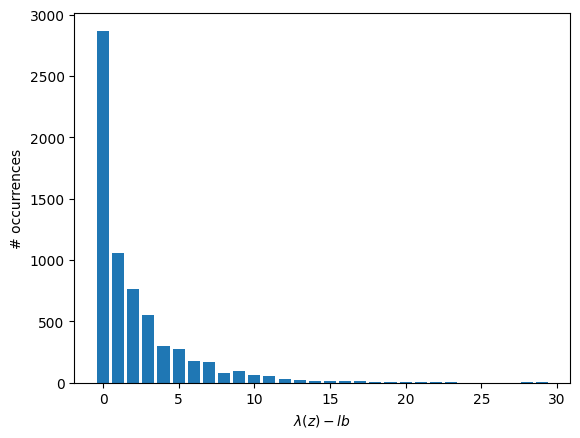
\includegraphics[width=\textwidth]{figures/LB0t2with012outliers.png}
            \end{figure}
        \end{column}
        \begin{column}{0.45\textwidth}
        \begin{center}
            $g = v$ primes.
        \end{center}
            \begin{figure}
                \centering
                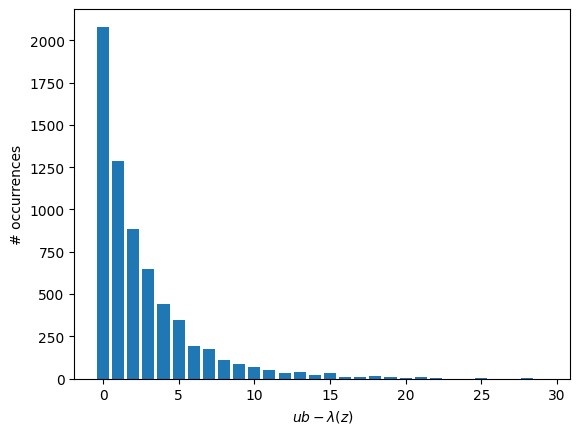
\includegraphics[width=\textwidth]{figures/UBt2with005outliers.png}
            \end{figure}
        \end{column}
    \end{columns}
    \begin{center}
                Distribution of $\rho(t+1)v/\rho(t)$ as a heatmap
    \end{center}
\end{frame}

\begin{frame}{ElGamal Sequences tuples lower and upper bounds}
    \begin{tabular}{ccc}
        a & Lower bounds & Upper bound \\
        $t = 2$ & 
        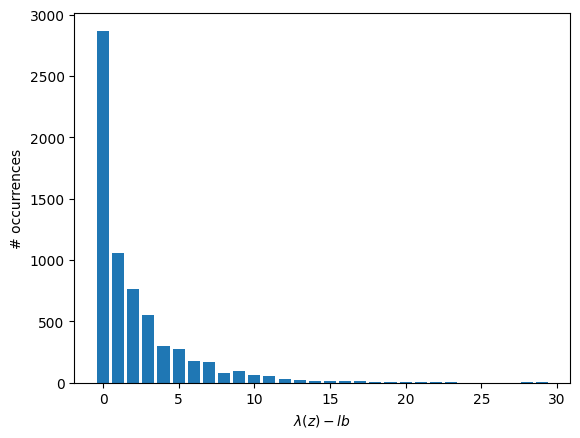
\includegraphics[width=0.3\textwidth]{figures/LB0t2with012outliers.png} &
        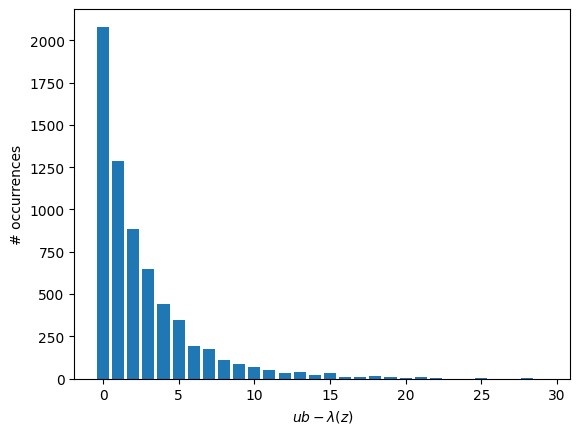
\includegraphics[width=0.3\textwidth]{figures/UBt2with005outliers.png} \\
        $t = 7$ & 
        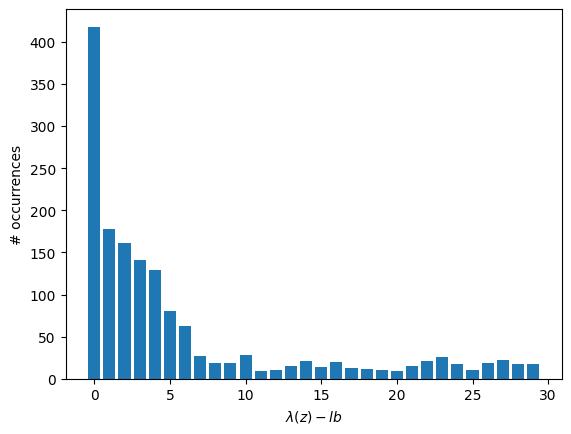
\includegraphics[width=0.3\textwidth]{figures/LB0t7with5975outliers.png} &
        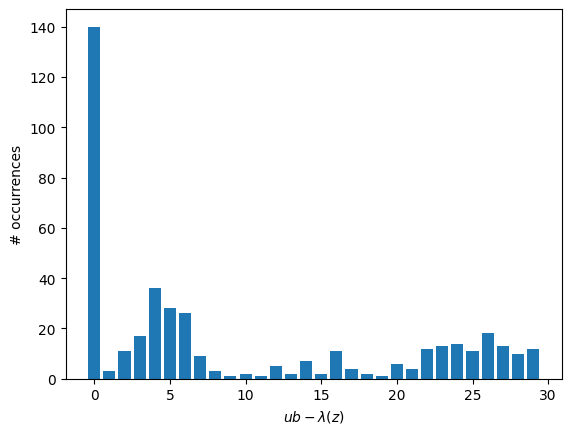
\includegraphics[width=0.3\textwidth]{figures/UBt7with9356outliers.png} 
    \end{tabular}
    \begin{center}
                Distribution of $\rho(t+1)v/\rho(t)$ as a heatmap
    \end{center}
\end{frame}

